\documentclass[11pt,a4paper]{article}

\usepackage[margin=2.5cm]{geometry}
\usepackage[T1]{fontenc}
\usepackage{lmodern}
\usepackage{amsmath}
\usepackage{graphicx}
\usepackage{float}
\usepackage{booktabs}
\usepackage{array}
\usepackage{caption}
\usepackage{subcaption}
\usepackage{enumitem}
\usepackage{xcolor}
\usepackage[colorlinks=true,linkcolor=blue!50!black,urlcolor=blue!50!black]{hyperref}

\graphicspath{{./}}
\setlength{\parskip}{0.5em}
\setlength{\parindent}{0pt}
\captionsetup{font=small,labelfont=bf}
\newcommand{\tbd}[1]{\textcolor{red}{\textbf{#1}}}

\title{Cascaded Voltage--Current Control of a\\Single-Phase Boost Power Factor Correction Converter}
\author{Aayush Singh - 24EEE1001\\[2pt]
Department of Electrical and Electronics Engineering\\
National Institute of Technology Goa}
\date{}
\begin{document}
\maketitle

\begin{abstract}
A single-phase diode-bridge rectifier followed by a boost converter is regulated at $415\,\mathrm{V}$ using cascaded control: an outer voltage loop sets the amplitude of a rectified-sine current reference, and the inner current loop drives the PWM generator. The designs were built and simulated in Simulink: a single-loop design with an SR latch, a cascaded design with a constant current reference, and a cascaded design whose current reference is shaped by the rectified input voltage. The final design starts from a discharged output capacitor, overshoots to about $480\,\mathrm{V}$ at $0.03\,\mathrm{s}$, and returns to $415\,\mathrm{V}$ by $0.5\,\mathrm{s}$. In steady state it holds about $1.2\,\mathrm{V}$ peak-to-peak output ripple ($0.3\%$) and draws a sinusoidal input current that is in phase with the source voltage.
\end{abstract}

%------------------------------------------------------------------
\section{Introduction and objectives}
The assignment asked for a boost converter with an outer and an inner control loop. The objectives adopted were:
\begin{itemize}[nosep]
  \item Regulate the DC output at $415\,\mathrm{V}$ from a single-phase AC source
  \item Implement a cascaded structure with an outer voltage loop and an inner inductor-current loop
  \item To make the input current sinusoidal and in phase with the source voltage (power factor correction)
  \item Keeping the startup transient, settling time and output ripple small
\end{itemize}
All work was done in Simulink with Simscape Electrical, using a discrete powergui.

%------------------------------------------------------------------
\section{System description}
The power stage is a diode-bridge rectifier feeding a boost converter whose MOSFET is gated by a PWM generator. The output diode feeds a parallel RC load. Table~\ref{tab:params} lists the parameters of the final design.

\begin{table}[H]
\centering
\caption{Parameters of the final design.}
\label{tab:params}
\begin{tabular}{@{}p{5.2cm}p{8.6cm}@{}}
\toprule
Parameter & Value \\
\midrule
AC source & single phase, $230\,\mathrm{V}$ peak ($\approx 163\,\mathrm{V}$ rms), $50\,\mathrm{Hz}$ \\
Rectifier & four diodes with snubbers, full bridge \\
Boost inductor $L$ & $3\,\mathrm{mH}$ \\
Output capacitor $C$ & $10\,\mathrm{mF}$ \\
Load resistor $R$ & $100\,\Omega$ \\
Output reference $V_\mathrm{ref}$ & $415\,\mathrm{V}$ \\
Outer PI & $K_{pv}=0.005$, $K_{iv}=0.05$; output limited to $0$--$600$; anti-windup: none \\
Inner PI & $K_{pi}=0.5$, $K_{ii}=100$; \\
PWM carrier frequency & $1000\,\mathrm{Hz}$ \\
Solver & discrete powergui, sample time $10^{-5}\,\mathrm{s}$ \\
Simulation stop time & $0.5\,\mathrm{s}$ for the cold-start captures; $2\,\mathrm{s}$ for the steady-state captures \\
\bottomrule
\end{tabular}
\end{table}
% TODO: fill in the PWM carrier frequency and the duty saturation limits from the model.

\paragraph{Operating point.} The output power is $P_o = V_\mathrm{ref}^2/R = 415^2/100 \approx 1.72\,\mathrm{kW}$, so the output current is $4.15\,\mathrm{A}$. With $V_\mathrm{rms}\approx 163\,\mathrm{V}$ and unity power factor the input rms current is $P_o/V_\mathrm{rms}\approx 10.6\,\mathrm{A}$, a fundamental peak of about $15\,\mathrm{A}$, neglecting losses.

%------------------------------------------------------------------
\section{Control architecture}
\label{sec:control}
With $d$ the duty cycle, $v_\mathrm{rect}=|v_s|$ the rectified bus voltage, $i_L$ the inductor current and $v_o$ the output voltage, the averaged boost model is
\begin{align}
L\,\frac{di_L}{dt} &= v_\mathrm{rect} - (1-d)\,v_o, \\
C\,\frac{dv_o}{dt} &= (1-d)\,i_L - \frac{v_o}{R}.
\end{align}

The controller has two nested loops, as follows.
\begin{enumerate}[nosep]
  \item \textbf{Outer voltage loop.} The error $e_v = V_\mathrm{ref}-v_o$ enters a PI controller followed by a saturation block, giving a conductance-like amplitude $u$:
  \begin{equation}
    u = K_{pv}\,e_v + K_{iv}\!\int e_v\,dt .
  \end{equation}
  \item \textbf{Current reference.} The rectified bus voltage is sensed before the inductor and multiplied by $u$:
  \begin{equation}
    i_\mathrm{ref}(t) = u(t)\,v_\mathrm{rect}(t).
  \end{equation}
  The reference is therefore a rectified sine whose amplitude is set by the voltage loop. This multiplier is what turns a plain cascaded regulator into a power factor corrector.
  \item \textbf{Inner current loop.} The error $e_i = i_\mathrm{ref}-i_L$ enters the inner PI, followed by a saturation block that limits the duty command:
  \begin{equation}
    d = \mathrm{sat}\!\left(K_{pi}\,e_i +   K_{ii}\!\int e_i\,dt\right).
  \end{equation}
  \item \textbf{PWM.} The PWM generator converts $d$ into gate pulses for the MOSFET.
\end{enumerate}

The outer loop is deliberately slow. The PI zero is at $K_{iv}/K_{pv}=10\,\mathrm{rad/s}$ ($\approx 1.6\,\mathrm{Hz}$), far below the $100\,\mathrm{Hz}$ ripple on the output capacitor, so the loop does not try to cancel that ripple, which would distort the input current. The inner PI zero is at $K_{ii}/K_{pi}=200\,\mathrm{rad/s}$ ($\approx 32\,\mathrm{Hz}$).

\paragraph{Consistency checks.} In steady state the average input power equals $P_o$, so $u = P_o/V_\mathrm{rms}^2 \approx 1720/163^2 \approx 0.065\,\mathrm{S}$. This is far below the outer upper limit of $600$, so that limit is inactive in steady state. The double-line-frequency output ripple is estimated by
\begin{equation}
  \Delta V_{pp} \approx \frac{P_o}{\omega_\mathrm{line}\,C\,V_o}
  = \frac{1722}{314\cdot 0.01\cdot 415} \approx 1.3\,\mathrm{V},
\end{equation}
which agrees with the $1.2\,\mathrm{V}$ read from the simulation (Section~\ref{sec:results}).

%------------------------------------------------------------------
\section{Design iterations}
Three designs were built and simulated. Values below are read from the scopes and meters.

\subsection{Design 1: single voltage loop with an SR latch}
A single PI output, after saturation, is compared with a ramp. A comparator drives the reset input of an SR latch and a pulse train drives the set input. The latch output gates the MOSFET (Fig.~\ref{fig:d1}). The design is simple, but the output settles at $413.5\,\mathrm{V}$, a $1.5\,\mathrm{V}$ steady-state error, and is still creeping upward at the end of the $6\,\mathrm{s}$ run.

\begin{figure}[H]
\centering
\begin{subfigure}{0.8\textwidth}
  \centering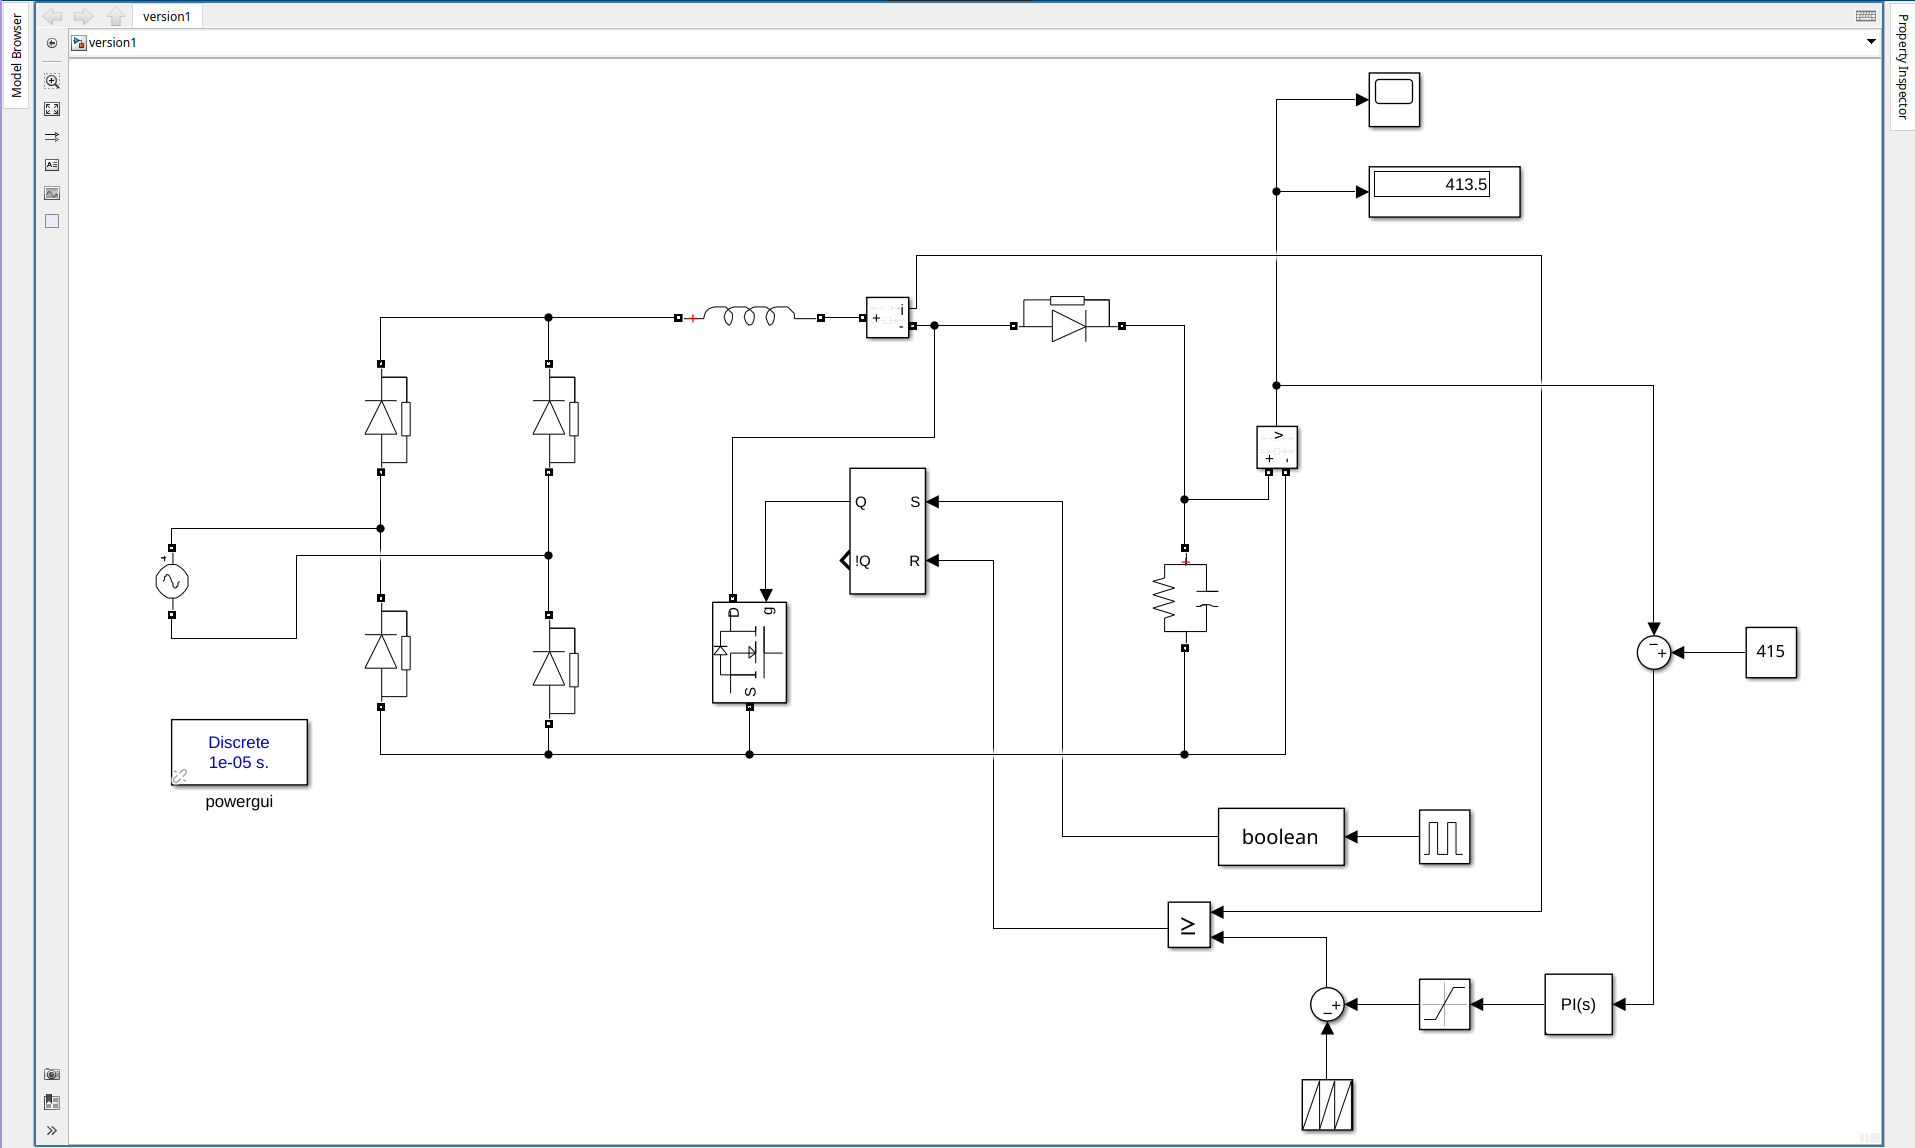
\includegraphics[width=\linewidth]{5.1a.png}
  \caption{Circuit and controller.}
\end{subfigure}\\[6pt]
\begin{subfigure}{0.8\textwidth}
  \centering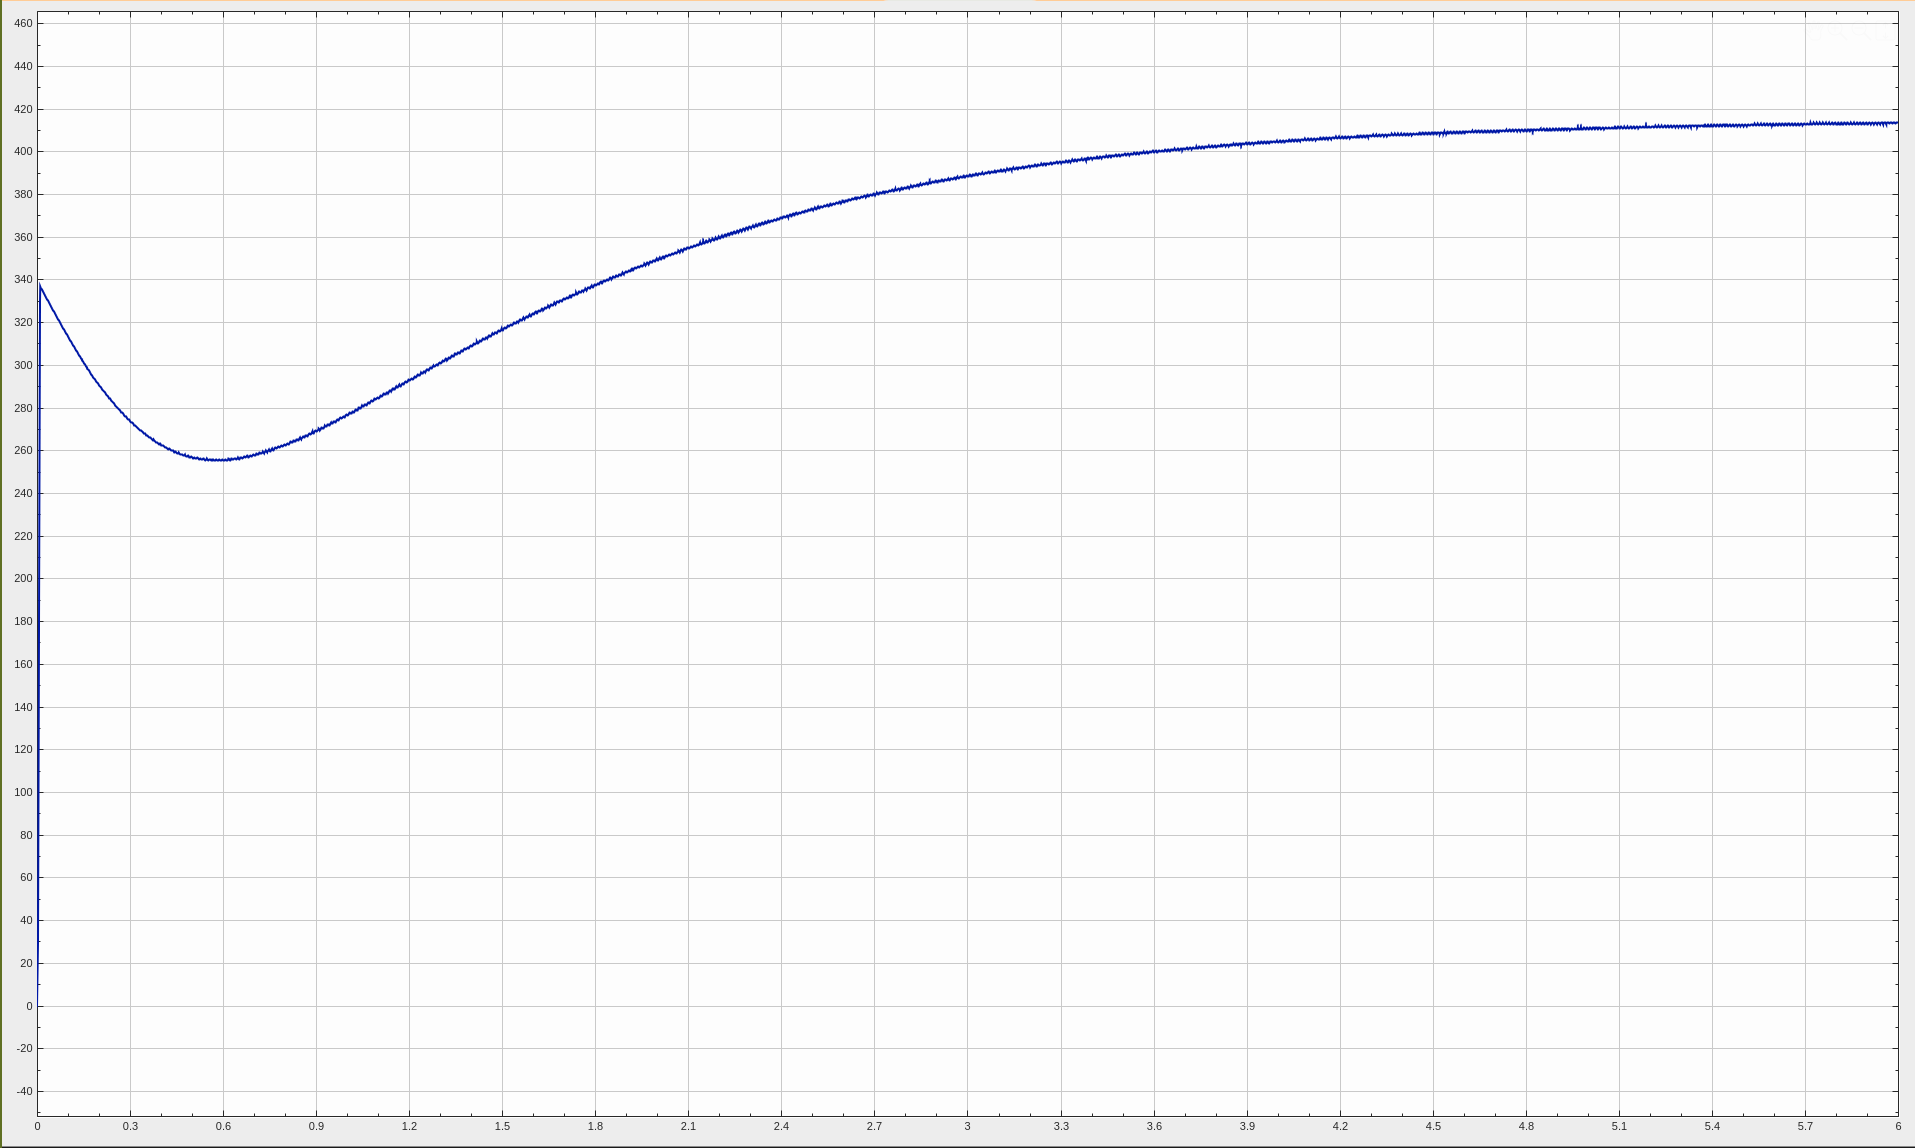
\includegraphics[width=\linewidth]{5.1b.png}
  \caption{Output voltage.}
\end{subfigure}
\caption{Design 1: single voltage loop with an SR latch.}
\label{fig:d1}
\end{figure}

\subsection{Design 2: cascaded loops with a constant current reference}
The second design has the outer voltage PI feeding an inner current PI and a PWM generator (Fig.~\ref{fig:d2}). It meets the brief of an outer and an inner loop and regulates more accurately ($414.9\,\mathrm{V}$), but the current reference has no shape, so the input current is not forced to follow the line voltage. The output dips to about $268\,\mathrm{V}$ at $0.55\,\mathrm{s}$, overshoots to about $419\,\mathrm{V}$ ($\approx 1\%$) and settles after about $7.5\,\mathrm{s}$.

\begin{figure}[H]
\centering
\begin{subfigure}{0.8\textwidth}
  \centering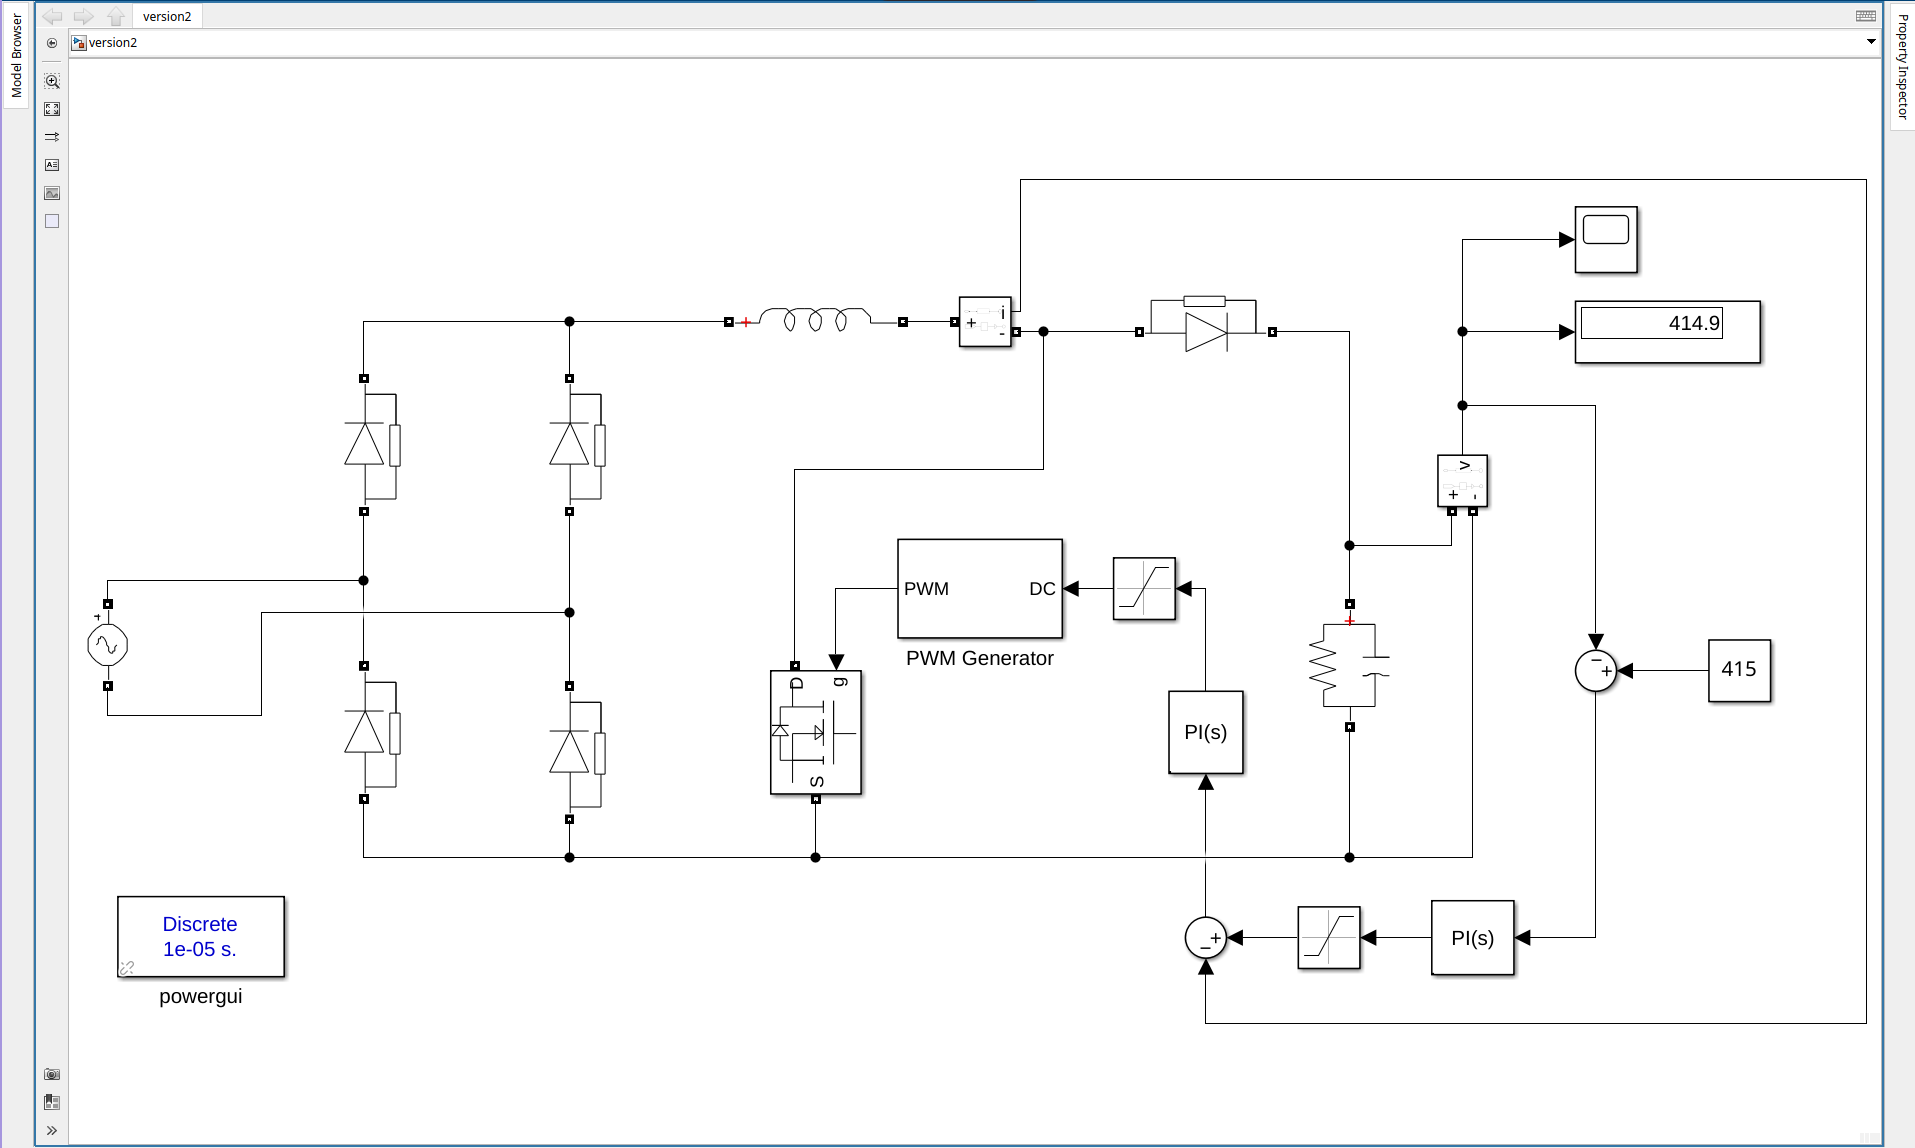
\includegraphics[width=\linewidth]{5.2a.png}
  \caption{Circuit and controller.}
\end{subfigure}\\[6pt]
\begin{subfigure}{0.8\textwidth}
  \centering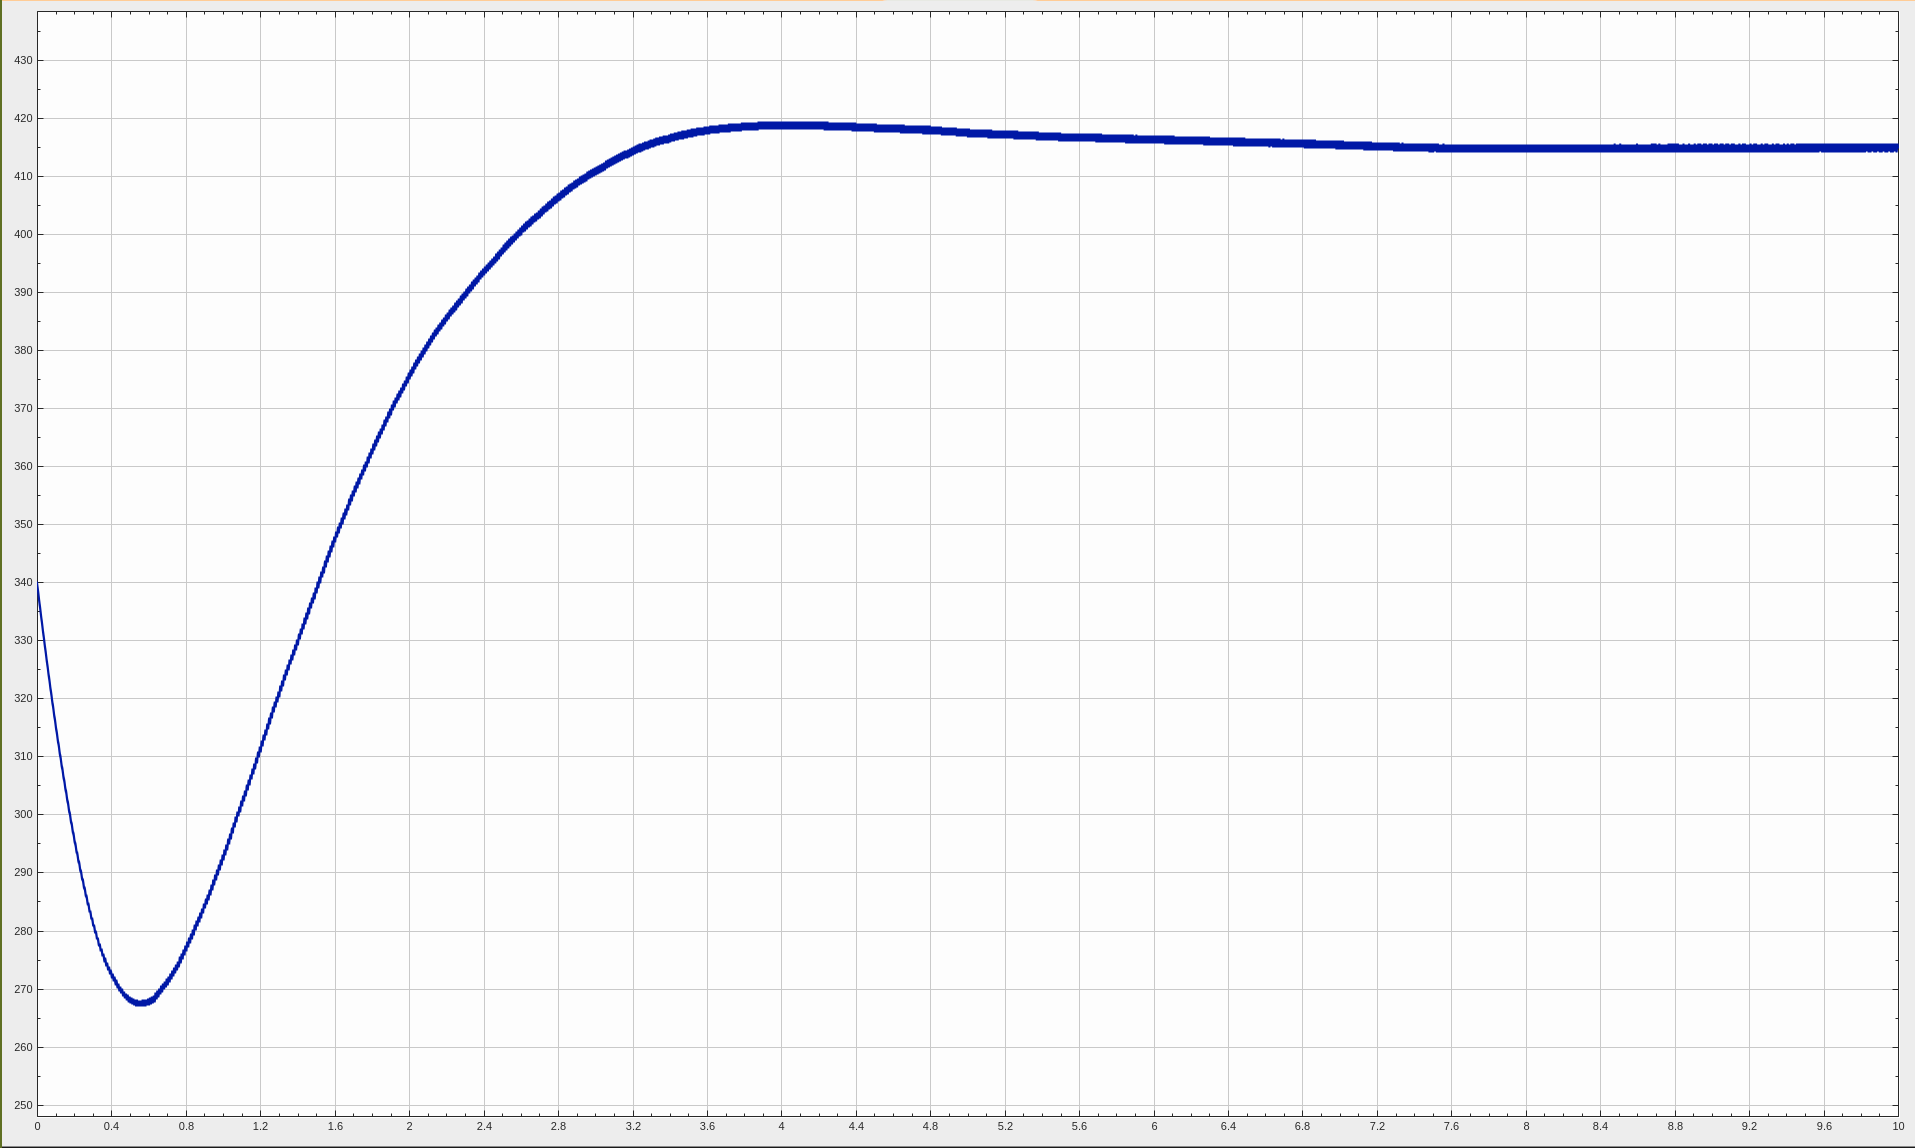
\includegraphics[width=\linewidth]{5.2b.png}
  \caption{Output voltage.}
\end{subfigure}
\caption{Design 2: cascaded voltage and current loops, constant current reference.}
\label{fig:d2}
\end{figure}

\subsection{Design 3: cascaded loops with a voltage-shaped current reference}
The final design adds the multiplier of Section~\ref{sec:control}, so the current reference follows the rectified line voltage (Fig.~\ref{fig:d3}). The loop gains were kept as in Table~\ref{tab:params}. The inductor was enlarged and the PWM carrier frequency raised to leave discontinuous conduction (Section~\ref{sec:issues}).

\begin{figure}[H]
\centering
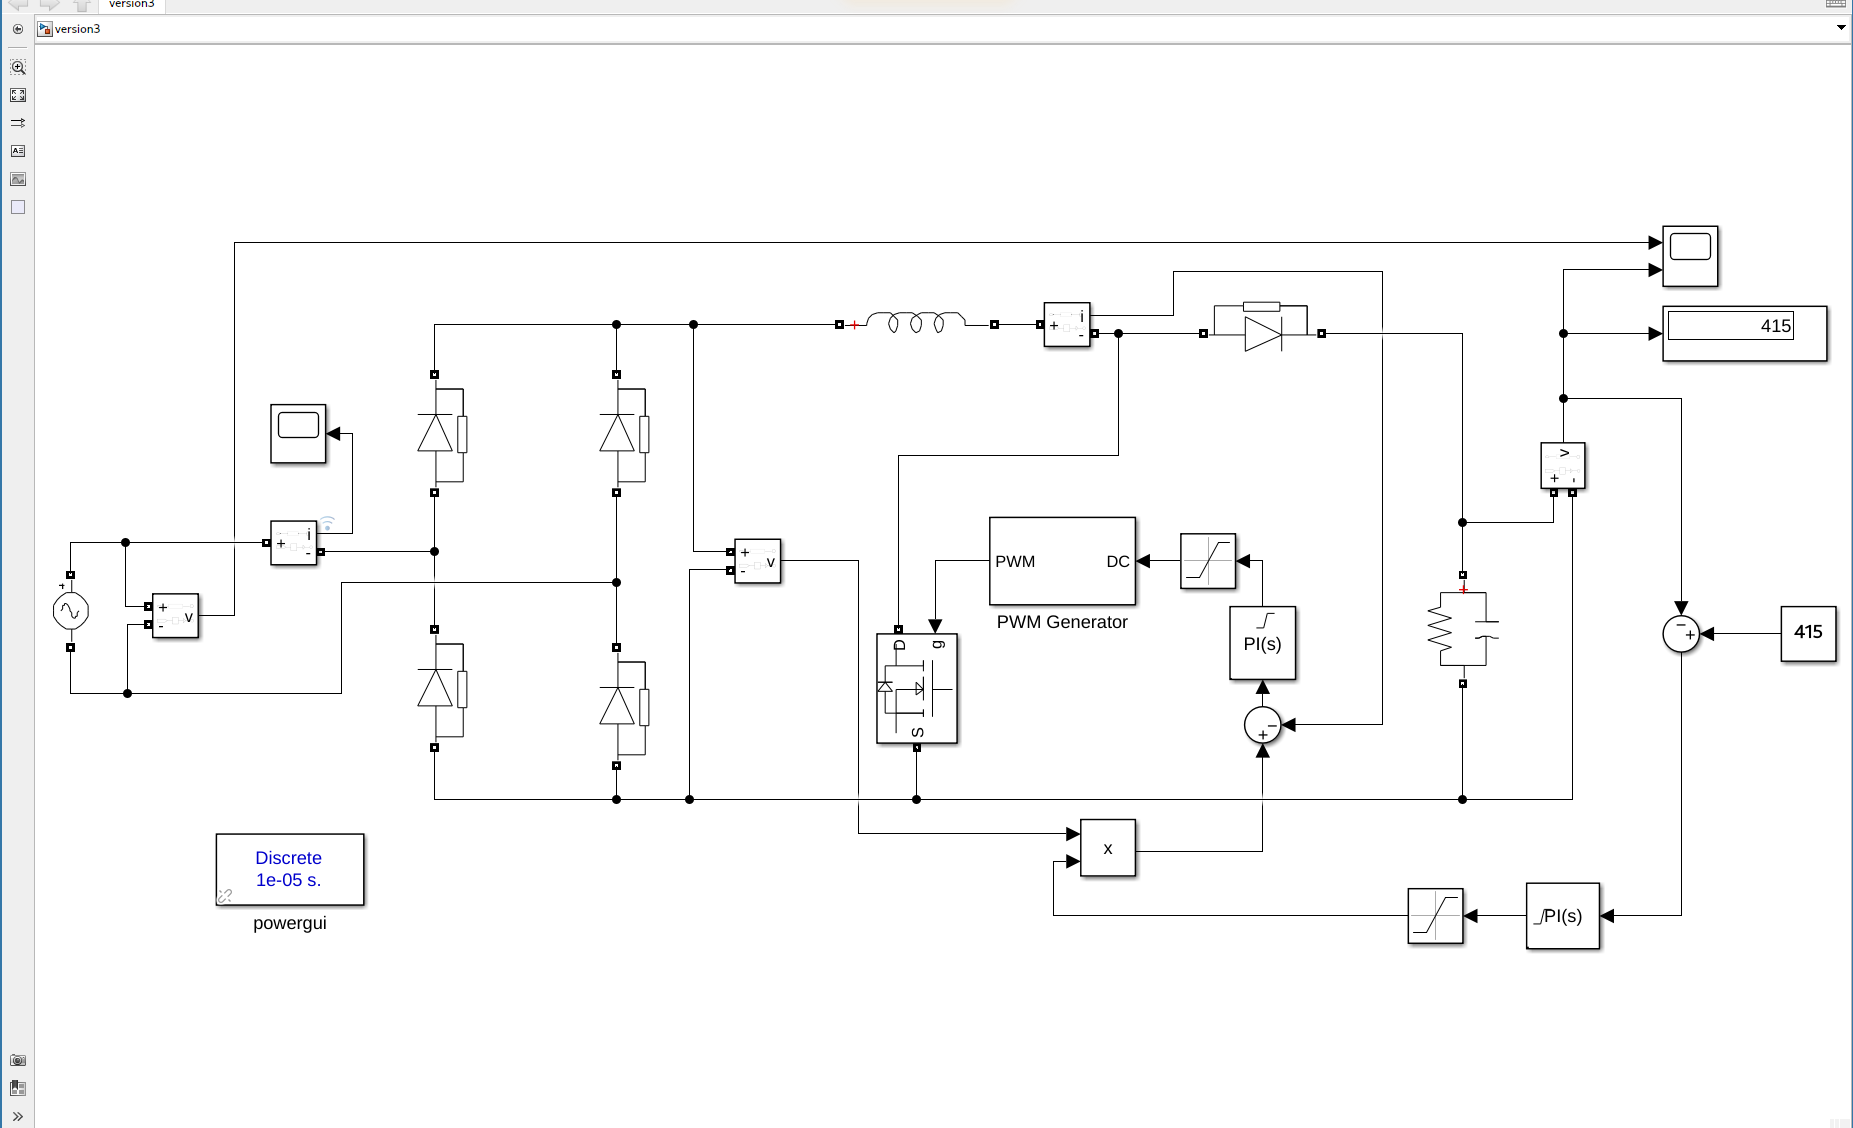
\includegraphics[width=\linewidth]{5.3a.png}
\caption{Design 3 (final): circuit and cascaded controller with the voltage multiplier. A voltage sensor and a current sensor on the source feed the scopes.}
\label{fig:d3}
\end{figure}

\begin{table}[H]
\centering
\caption{Comparison of the three designs, read from the scopes.}
\label{tab:compare}
\begin{tabular}{@{}>{\raggedright\arraybackslash}p{2.2cm}>{\raggedright\arraybackslash}p{4.6cm}>{\raggedright\arraybackslash}p{2.4cm}>{\raggedright\arraybackslash}p{4.2cm}@{}}
\toprule
Design & Control structure & Final output & Observations \\
\midrule
1 & single PI, SR latch, ramp & $413.5\,\mathrm{V}$ & starts at $\approx 340\,\mathrm{V}$, dips to $\approx 255\,\mathrm{V}$; slow, still rising at $6\,\mathrm{s}$ \\
2 & cascaded PIs, constant current reference & $414.9\,\mathrm{V}$ & starts at $\approx 340\,\mathrm{V}$, dips to $\approx 268\,\mathrm{V}$; overshoot $\approx 4\,\mathrm{V}$; settles in $\approx 7.5\,\mathrm{s}$ \\
3 & cascaded PIs, voltage-shaped reference & $415\,\mathrm{V}$ & cold start from $0\,\mathrm{V}$; overshoot to $\approx 480\,\mathrm{V}$; at $415\,\mathrm{V}$ by $0.5\,\mathrm{s}$ \\
\bottomrule
\end{tabular}
\end{table}

The startup rows are not like-for-like: the Design~1 and 2 scopes start near $340\,\mathrm{V}$, while the Design~3 capture starts from a discharged capacitor.

%------------------------------------------------------------------
\section{Results of the final design}
\label{sec:results}

\subsection{Cold-start transient}
Figure~\ref{fig:startvolt} shows the source voltage and the output voltage from a discharged output capacitor. The output rises to about $480\,\mathrm{V}$ at $0.03\,\mathrm{s}$, an overshoot of about $16\%$, then decays slowly to about $442\,\mathrm{V}$ at $0.12\,\mathrm{s}$, about $419\,\mathrm{V}$ at $0.3\,\mathrm{s}$, and $415\,\mathrm{V}$ at $0.5\,\mathrm{s}$.

\begin{figure}[H]
\centering
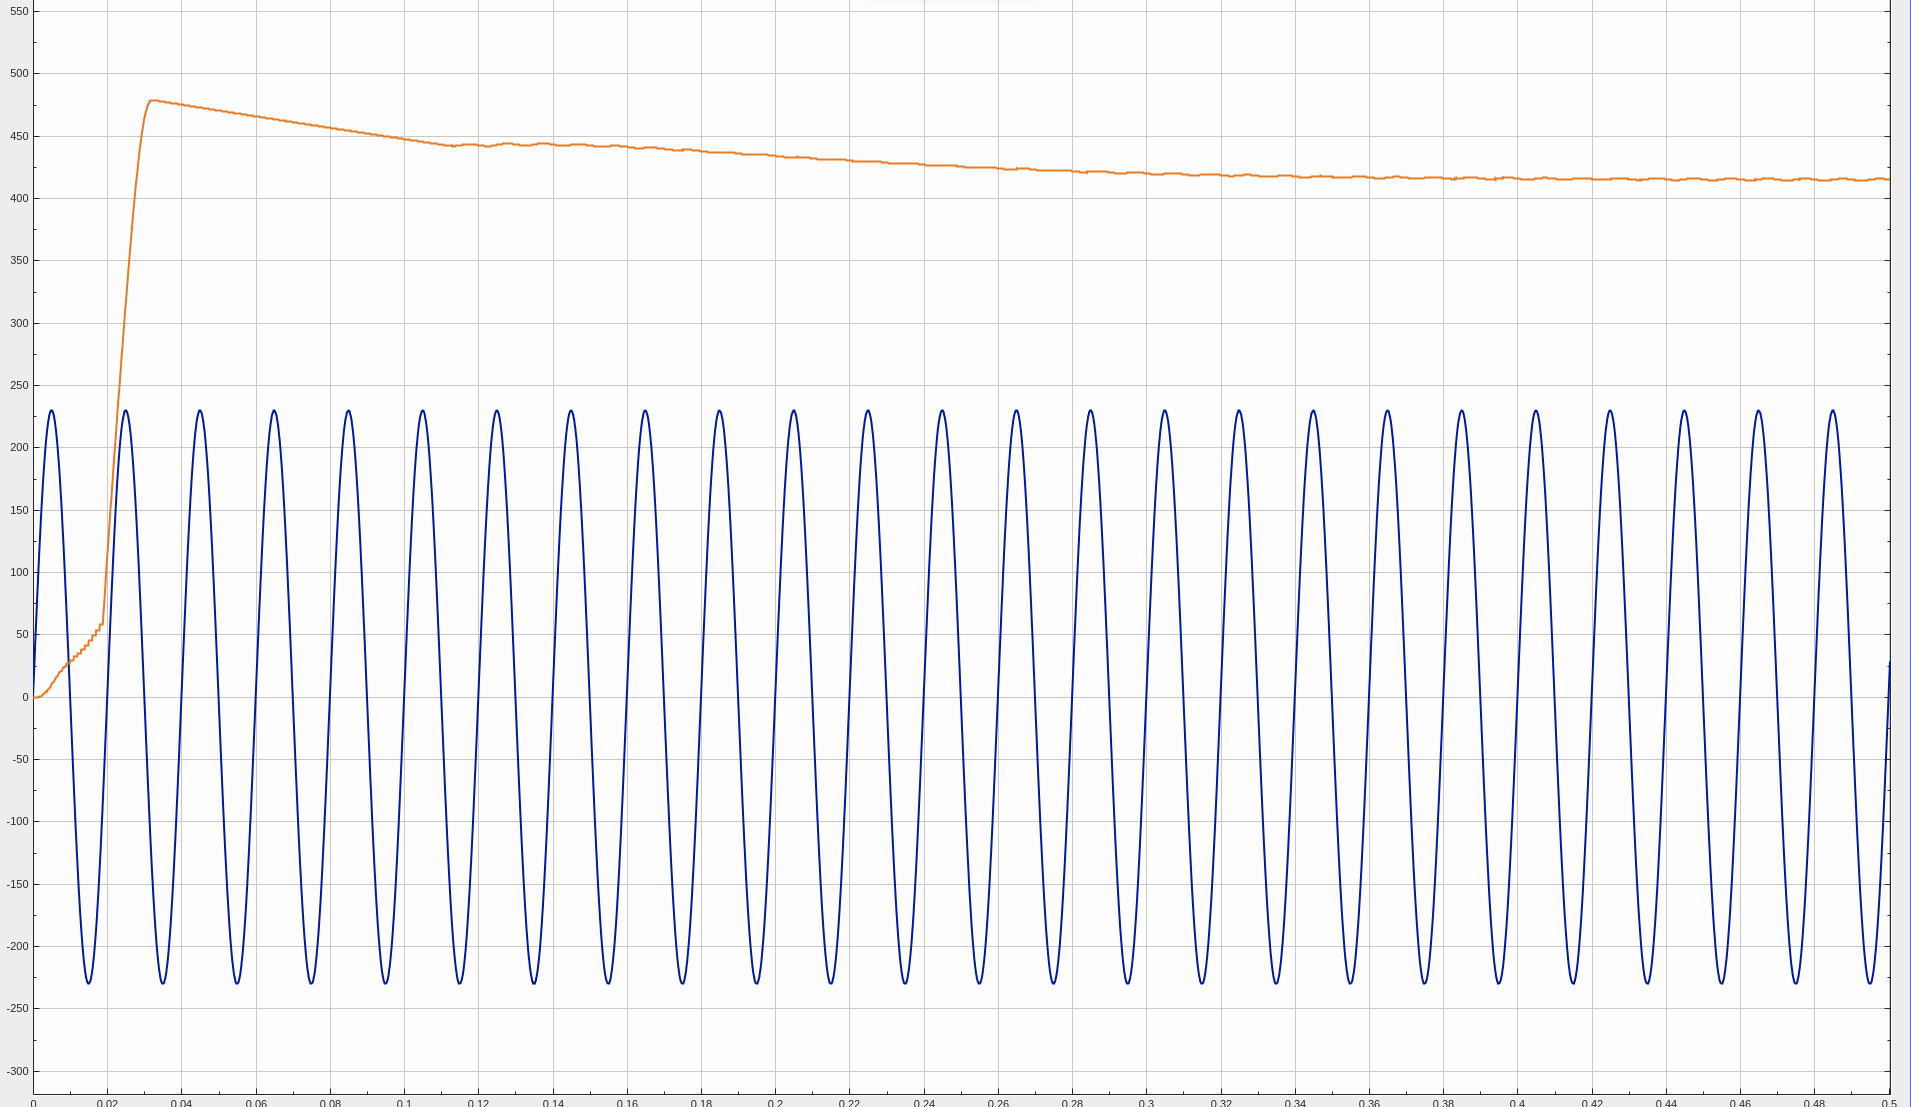
\includegraphics[width=0.92\linewidth]{5.3b.png}
\caption{Cold start: source voltage (blue, $230\,\mathrm{V}$ peak) and output voltage (yellow), $0$--$0.5\,\mathrm{s}$.}
\label{fig:startvolt}
\end{figure}

Figure~\ref{fig:startcur} shows the source current over the same window. During the first $0.03\,\mathrm{s}$ the current has large inrush spikes, of the order of hundreds of amperes, while the capacitor charges through an ideal source. The size of the peak is consistent with the outer loop: at $t=0$ the voltage error is $415\,\mathrm{V}$, so the proportional term alone gives $K_{pv}\,e_v\,v_\mathrm{rect}\approx 0.005\cdot 415\cdot 230\approx 480\,\mathrm{A}$, close to the observed peaks of about $470$--$480\,\mathrm{A}$, and the outer upper limit of $600$ does not restrict it. The current is then close to zero until about $0.11\,\mathrm{s}$, while the output is above its reference. After that a $50\,\mathrm{Hz}$ sinusoid appears, starting at about $25\,\mathrm{A}$ peak and shrinking towards the steady-state value.

\begin{figure}[H]
\centering
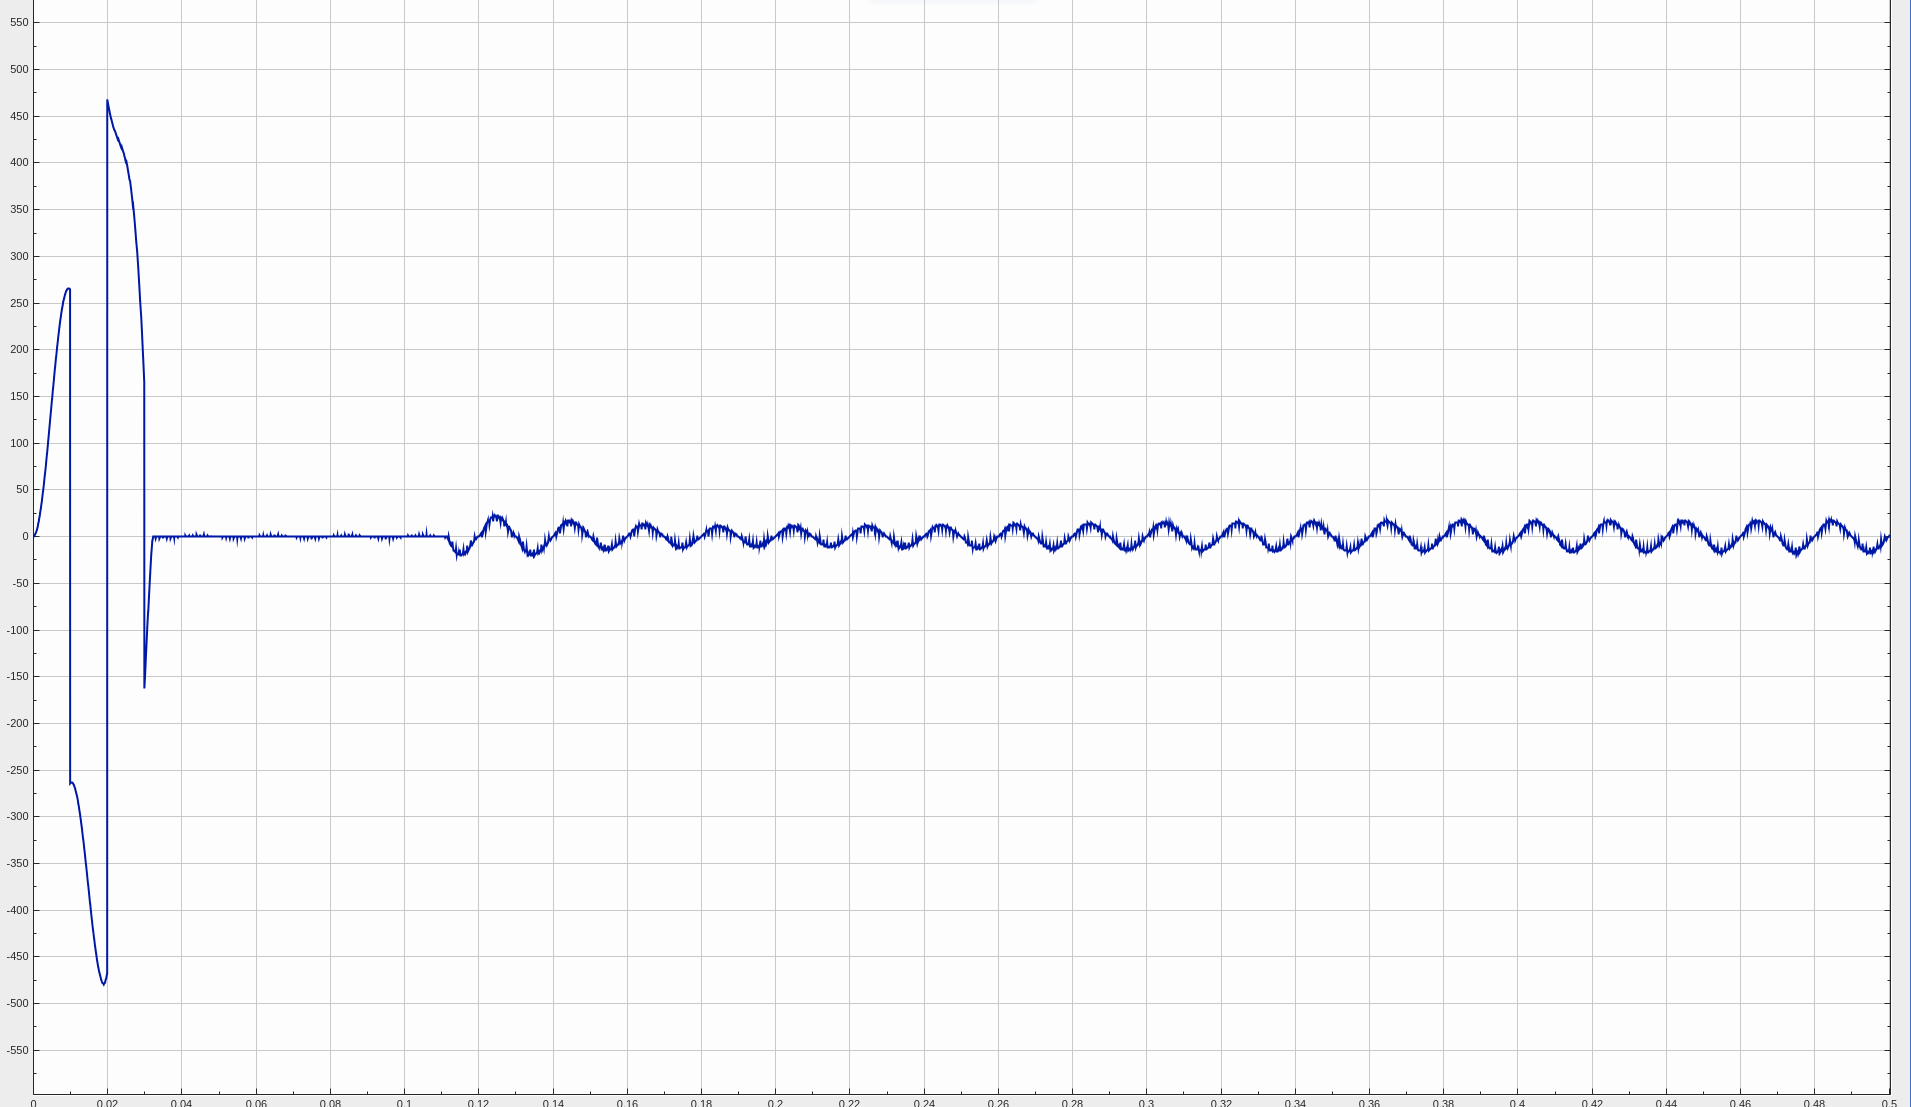
\includegraphics[width=0.92\linewidth]{5.3c.png}
\caption{Cold start: source current, $0$--$0.5\,\mathrm{s}$.}
\label{fig:startcur}
\end{figure}

The pause in current is consistent with the outer PI sitting on its lower limit while the output is above the reference, with anti-windup disabled delaying recovery. This explanation was not tested.

\subsection{Steady state}
Figure~\ref{fig:ss} shows the source voltage and the source current at steady state. The current is a sinusoid with switching ripple riding on it, and its peaks and zero crossings line up with those of the voltage, which indicates near-unity power factor. The measured envelope is about $15\,\mathrm{A}$ with spikes up to about $18\,\mathrm{A}$, close to the $15\,\mathrm{A}$ expected from the power balance. The current is flat close to the zero crossings, the usual low-voltage distortion of a boost PFC stage.

\begin{figure}[H]
\centering
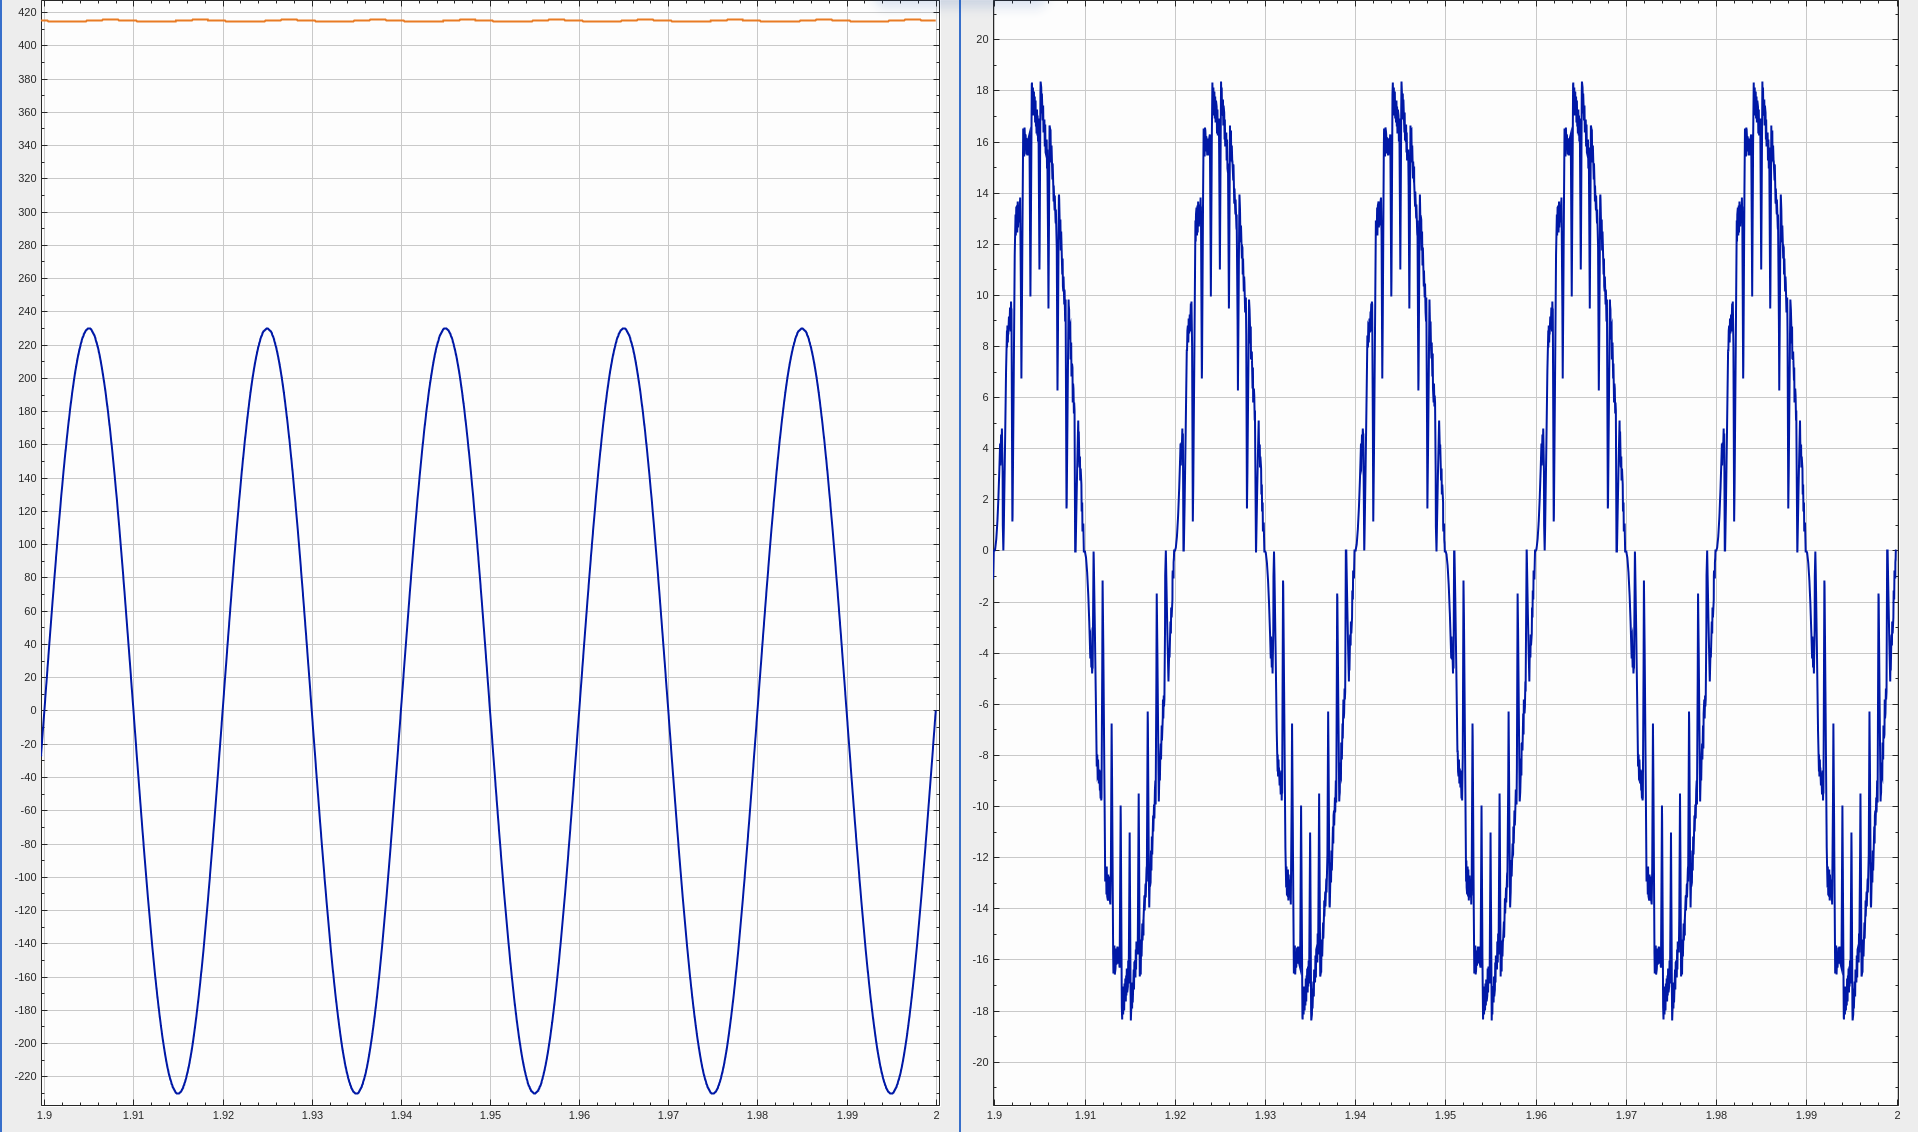
\includegraphics[width=\linewidth]{5.3d.png}
\caption{Steady state, $1.9$--$2\,\mathrm{s}$: source voltage and output voltage (left), source current (right).}
\label{fig:ss}
\end{figure}

The output voltage ripple is shown in Fig.~\ref{fig:ripple}: a $100\,\mathrm{Hz}$ wave between about $414.4\,\mathrm{V}$ and $415.6\,\mathrm{V}$, i.e.\ $1.2\,\mathrm{V}$ peak to peak or $0.3\%$. This is the expected price of power factor correction in a single-phase system, since the instantaneous input power pulsates at twice the line frequency while the load draws constant power.

\begin{figure}[H]
\centering
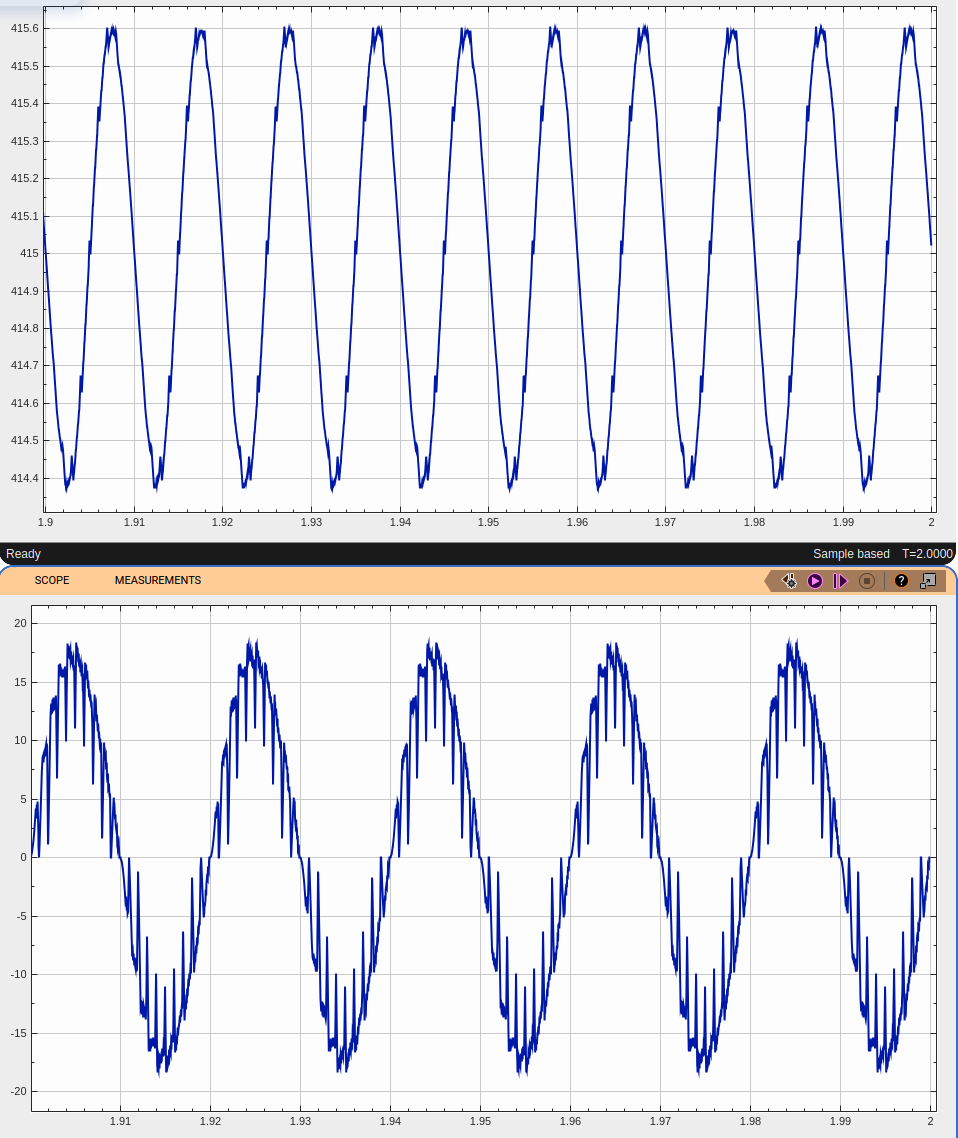
\includegraphics[width=0.75\linewidth]{5.3e.png}
\caption{Steady-state output voltage ripple.}
\label{fig:ripple}
\end{figure}

\begin{table}[H]
\centering
\caption{Summary of the final design.}
\label{tab:results}
\begin{tabular}{@{}p{5cm}p{8.8cm}@{}}
\toprule
Metric & Result \\
\midrule
Steady-state output & $415\,\mathrm{V}$ (target $415\,\mathrm{V}$) \\
Output ripple & $\approx 1.2\,\mathrm{V}$ peak to peak ($0.3\%$) at $100\,\mathrm{Hz}$ \\
Cold-start overshoot & $\approx 480\,\mathrm{V}$ at $0.03\,\mathrm{s}$ ($\approx 16\%$) \\
Return to reference & $\approx 0.5\,\mathrm{s}$ \\
Inrush current & hundreds of amperes in the first $0.03\,\mathrm{s}$ (ideal source) \\
Steady-state input current & sinusoidal, $\approx 15\,\mathrm{A}$ envelope, continuous conduction \\
Phase & current peaks and zero crossings align with the source voltage \\
\bottomrule
\end{tabular}
\end{table}

%------------------------------------------------------------------
\section{Issues encountered and fixes}
\label{sec:issues}

\begin{table}[H]
\centering
\caption{Problems found during development.}
\label{tab:issues}
\begin{tabular}{@{}>{\raggedright\arraybackslash}p{3.3cm}>{\raggedright\arraybackslash}p{4.2cm}>{\raggedright\arraybackslash}p{3.5cm}>{\raggedright\arraybackslash}p{2.8cm}@{}}
\toprule
Symptom & Cause & Fix & Outcome \\
\midrule
Output stuck at $233\,\mathrm{V}$ & a squaring block after the multiplier made the reference the square of the product, not a rectified sine, so the converter acted as a plain rectifier & removed the squaring block; multiplier wired straight to the inner summer & output reached $415\,\mathrm{V}$ \\
Output ran away to $1460\,\mathrm{V}$ & summer sign reversed during debugging, giving positive feedback & restored the original sign & stable regulation \\
Input current chopped to zero between spikes, up to $\approx 25\,\mathrm{A}$ & discontinuous conduction: inductor too small or carrier frequency too low & enlarged the inductor ($L=3\,\mathrm{mH}$) and raised the carrier frequency & continuous sinusoidal current \\
FFT tool showed an empty signal list & scope data was not logged as a structure with time & not resolved & THD not measured \\
\bottomrule
\end{tabular}
\end{table}

Figure~\ref{fig:dcm} shows the source current while the converter was in discontinuous conduction, before the inductor and carrier frequency were changed.

\begin{figure}[H]
\centering
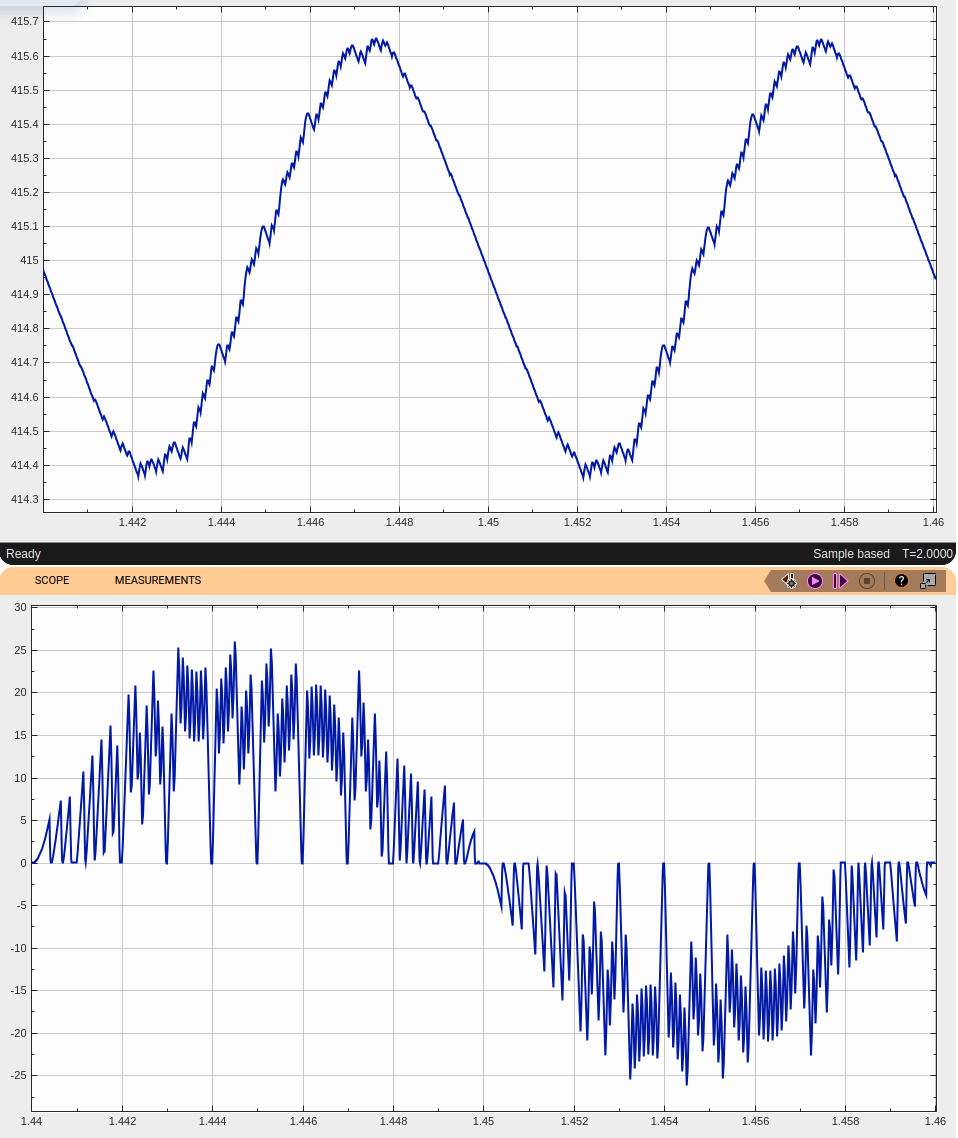
\includegraphics[width=0.75\linewidth]{5.3f.png}
\caption{Source current in discontinuous conduction, before the fix.}
\label{fig:dcm}
\end{figure}

%------------------------------------------------------------------
\section{Limitations and future work}
\begin{itemize}[nosep]
  \item \textbf{No THD figure.} Power factor and distortion were judged from waveforms only. Logging the source current to the workspace as a structure with time, and running the powergui FFT with a $50\,\mathrm{Hz}$ fundamental, would give a number; below about $5\%$ would be a good result.
  \item \textbf{Startup overshoot and inrush.} The $480\,\mathrm{V}$ cold-start overshoot and the inrush current need a soft-start reference ramp, anti-windup on both PI blocks, and an inrush limit or pre-charge circuit. Since $i_\mathrm{ref}=u\,v_\mathrm{rect}$, lowering the outer upper limit from $600$ to about $0.1\,\mathrm{S}$ (roughly $23\,\mathrm{A}$ at $230\,\mathrm{V}$ peak, about $1.5\times$ the expected $15\,\mathrm{A}$) would cap the reference directly. The model has no source impedance or pre-charge circuit visible in the diagram.
  \item \textbf{Like-for-like startup comparison.} Designs~1 and 2 should be rerun from the same initial condition as Design~3.
  \item \textbf{Load and line steps} were not tested, so robustness to load change and line variation is unverified.
  \item \textbf{Inner-loop bandwidth} was not checked against the carrier frequency. A first-order estimate, assuming unit PWM gain and ideal sensing, gives a crossover near $K_{pi}V_o/L\approx 7\times 10^4\,\mathrm{rad/s}$ ($\approx 11\,\mathrm{kHz}$), which should be compared with the carrier frequency; the residual switching ripple on the current may be reduced by retuning the inner PI or raising the carrier frequency.
  \item \textbf{Parameter completeness.} The PWM carrier frequency and the duty saturation limits should be added to Table~\ref{tab:params}.
\end{itemize}

%------------------------------------------------------------------
\section{Conclusion}
The cascaded design with a voltage-shaped current reference regulates the output at $415\,\mathrm{V}$ with $0.3\%$ ripple and draws a sinusoidal input current in phase with the source voltage, which meets the brief and is clearly better than the single latch-based loop and the unshaped cascaded design.

\end{document}
